\section{Chicken watch guard}\label{sec:chicken-watch-guard}
Služba Chicken Watch Guard je dalším klíčovým prvkem systému Coopmaster.
Poskytuje data o počtu slepic v kurníku a tato data předává do systému Home Assistant.\newline

\subsection*{Obecný princip}
Podobně jako u služby Dog Alarm, Chicken Watch Guard používá kamerový systém pro získávání aktuálních záběrů z kurníku.
Tyto záběry jsou staženy ze služby Camera Driver~\ref{sec:camera-driver}.
Získané obrázky se analyzují modelem Yolov11, který je upravený pro přesnější detekci v našich lokálních podmínkách.
Výsledky detekce společně s aktuální fotografií jsou pomocí protokolu MQTT odeslány do systému Home Assistant, který je využije při automatizaci dvířek a vizualizuje v uživatelském rozhraní.

\subsection*{Popis algoritmu}
Jako první je vytvořeno API definované pomocí Flask frameworku pro komunikaci se službou Health Checker.
Následně je inicializován a spuštěn scheduler, který má za úkol jednou za minutu spustit job s názvem check\_chicken.
Závěrem spouštěcí metody se spustí propagace API na portu 9003, který je předáván jako proměnná prostředí při startu služby.

\subsection*{Popis algoritmu pro počítání slepic}
Po spuštění se jako první provolá metoda get\_image, která je zodpovědná za stažení aktuálního obrázku ze služby Camera Driver.
Dále je inicializován detekční upravený model Yolov11 a provedena detekce objektů v obraze (sekce~\ref{sec:detekce-objektu-pomoci-strojoveho-uceni}).
Výsledkem je seznam objektů, které se podařilo identifikovat.
Hlavními daty, která obsahuje jedna položka v seznamu, jsou informace o detekované kategorii a oblast v obraze, kde přesně byl objekt nalezen.
Počet slepic v kurníku je dán počtem, kolikrát se v seznamu výskytuje kategorie slepice.
Job končí publikováním výsledného počtu slepic na MQTT topic coopmaster/chicken/count
 a aktuální fotografie (obrázek~\ref{fig:foto_z_guarda}) na MQTT topic coopmaster/chicken/image/actual.
Systém Home Assistant je MQTT subscriber zmíněných topics a reaguje na ně, jak je popsáno v sekci~\ref{sec:tvorba-gui-rozhrani}.

\begin{figure}[H]
    \centering
    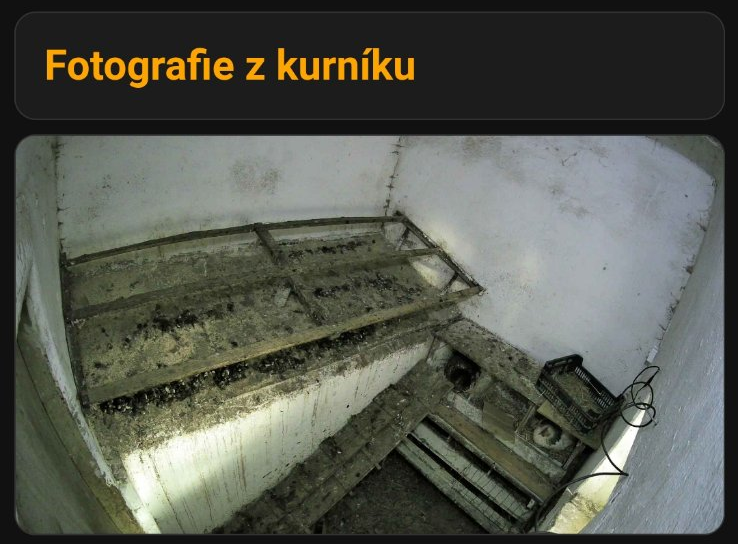
\includegraphics[width=0.8\textwidth]{img/foto_z_guarda}
    \caption{Obrázek přijatý z MQTT a vizualizovaný v dashboardu}
    \label{fig:foto_z_guarda}
\end{figure}

%\subsection*{Výhody a přínosy}
%
%Implementace služby Chicken Watch Guard přináší do systému Coopmaster následující výhody:
%\begin{itemize}
%    \item \textbf{Přesný monitoring:} Automatizovaný systém poskytuje přesné a aktuální informace o počtu slepic, což napomáhá efektivnímu plánování a rozhodování.
%    \item \textbf{Reálný čas přehledu:} Díky integraci s Home Assistanta je zajištěno promptní informování o změnách v kurníku, což umožňuje rychlou reakci.
%    \item \textbf{Vizualizace stavu:} Průběžné vizuální sledování přispívá k lepšímu porozumění a řízení prostředí v kurníku.
%\end{itemize}
%Úkolem služby Chicken watch guard je sledovat stav a počet slepic v kurníku.\newline
%Aktuální záběry jsou stejně jako u Dog alarmu stahovány z konkrétního Camera driveru v kurníku.
%Následně po získání záběru proběhne detekce objektů a počet těchto objektů udává počet detekovaných slepic v obraze.
%Tato hodnota je publikována pomocí MQTT do Home Assistanta.
%Vedlejší funkcí služby je průběžné posílání aktuálního pohledu z kamery v kurníku do Home Assistanta.
